\section{Gearing}\label{robot:gearing}
I \cref{sensorer:motorer} fandt vi ud af at præcisionen på motorerne ikke var høj.
Der var en afvigelse på op til 4\dg, imod en forventet afvigelse på max. 1\dg.
Dette faktum samt kravene fra \cref{robot:design} gav anledning til at udforske mulighederne for at geare motorene for at mindske denne præcision.

\subsection{Simpel Teori}\label{gearing:simpel_teori}
Gearing kan foregå på to måder; geare op eller geare ned.
Det tandhjul der er knyttet direkte til motoren kalder vi fører-tandhjulet og det tandhjul der er knyttet til fører-tandhjulet kalder vi for følger-tandhjulet (se evt. \cref{gearing:nedgearing}).

\subsubsection{Nedgearing}
Nedgearing foregår ved at et mindre tandhjul driver et større tandhjul.
Ratio'en (størrelsen af gearing) er styret af antallet af tænder på tandhjulene.
For eksempel vil et 24-tands fører-tandhjul drive et 40-tands følger-tandhjul med ratio'en $\frac{40}{24}$, hvilket betyder at der går 40 fører omdrejninger pr. 24 følger omdrejninger. Dvs. at motoren der driver fører-tandhjulet skal rotere $\frac{40}{24} = \frac{1 \frac{2}{3}}{1}$ omgange for at rotere følger-tandhjulet én omgang.

\begin{figure}[h]
\centering

\includegraphics[width=.5\textwidth]{gears/op_og_ned}
\caption{Eksempel på (ned-)gearing}
\label{gearing:nedgearing}
\end{figure}

\subsection{Aktuelle gearing}
Dette afsnit fokuserer på den teoretiske gearing for henholdsvis ultrasonisk sensor og hjul.
\Cref{robot:gearing-test} beskriver forskellige test af begge gearinger for at undersøge om de lever op til de teoretiske værdier.


\subsubsection{Ultrasonisk sensor}
Denne bruges til at bestemme tilkendegivelse og afstand af et objekt i en bestemt retning, hvorfor det vil være en klar fordel at geare motoren ned for at opnå større præcision af denne når retningen af sensoren skal bestemmes.
Rotationen vil naturligvis foregå langsommere end uden gearing, men tid er ikke en faktor på nuværende tidspunkt

Gearingen for den ultrasoniske sensor består af i alt 4 tandhjul, som alle kan ses i \cref{gearing:tandhjul}.

\begin{figure}[h] % De anvendte tandhjul
\centering
\begin{subfigure}[b]{.19\textwidth}
\centering
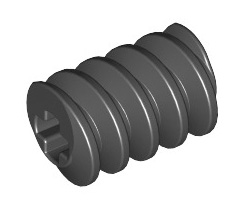
\includegraphics[width=\textwidth]{gears/worm}
\caption{Orm}
\label{gearing:orm}
\end{subfigure}
\begin{subfigure}[b]{.19\textwidth}
\centering

\includegraphics[width=\textwidth]{gears/16-tooth}
\caption{16-tands}
\label{gearing:16tand}
\end{subfigure}
\begin{subfigure}[b]{.19\textwidth}
\centering

\includegraphics[width=\textwidth]{gears/24-tooth}
\caption{24-tands}
\label{gearing:24tand}
\end{subfigure}
\begin{subfigure}[b]{.19\textwidth}
\centering
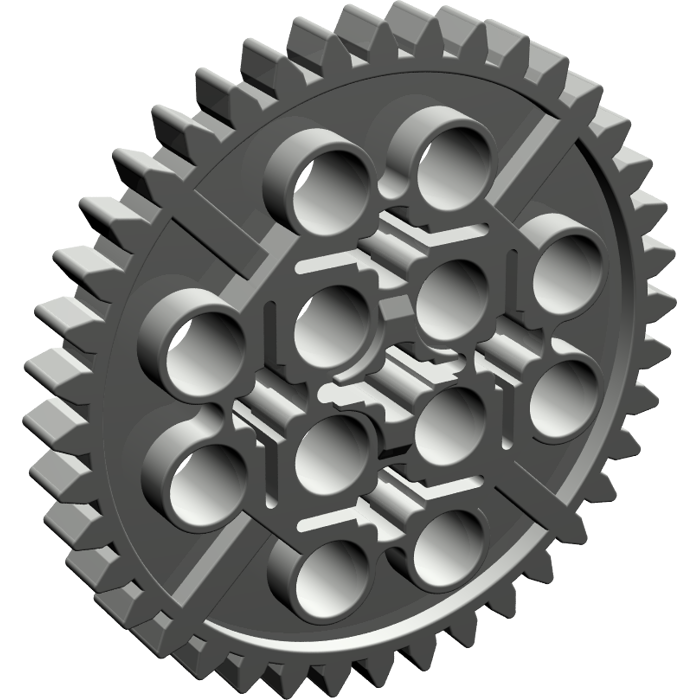
\includegraphics[width=\textwidth]{gears/40-tooth}
\caption{40-tands}
\label{gearing:40tand}
\end{subfigure}
\caption{De anvendte tandhjul for sensor og hjul}
\label{gearing:tandhjul}
\end{figure}

Den første kombination består af en orm (se \cref{gearing:orm}) som fører-tandhjul og 40-tands (se \cref{gearing:40tand}) som følger-tandhjul.
Ormen kræver en hel rotation for at flytte én tand på følger-tandhjul.
Dette giver en ratio på $\frac{40}{1} = 40$, hvilket betyder at der kræves 40 hele motor-rotationer for at rotere 40-tands tandhjulet én omgang.

Den anden kombination består af en 24-tands (se \cref{gearing:24tand}) som fører-tandhjul og en 56-tands (se \cref{gearing:56tand}) som følger-tandhjul.
Dette giver en ratio på $\frac{56}{24} = \frac{2\frac{1}{3}}{1}$.

Den samlede gearing for sensoren ser derfor således: $$\frac{40}{1} \cdot \frac{2\frac{1}{3}}{1} = \frac{93 \frac{1}{3}}{1}$$

\subsubsection{Hjul}
Motorene som styrer hjulsættet er ligesom sensoren også drevet af en gearing som gearer motorens omdrejninger ned, hvilket resulterer i to faktorer for kontrol af robotten:

\begin{itemize}
\item Højere præcision og mindskning af usikkerheder ved rotation af hjulene.
\item Højere moment af motorene som driver hjulene, hvilket gør det muligt at kontrollere robotten ved lavere hastigheder samt kørsel på underlag med høj friktion.
\end{itemize}

Igen er tid ikke en faktor, så det er acceptabelt at robotten mister fart.
Præcision af motorernes position er ikke af væsentlig faktor, da robottens lokationen bestemmes andetsteds og ikke vha. \textit{dead reckoning}.

Gearingen for hjulene består hver især af to tandhjul; ét 40-tands og ét 24-tands.
Derved er gearingen som i eksemplet i \cref{gearing:simpel_teori}: $$ \frac{40}{24} = 1 \frac{2}{3} $$

\subsection{Test af gearing}\label{robot:gearing-test}
Nu hvor den teoretiske gearing er fastlagt, vil der her blive udført en række forsøg for at afgøre præcisionen af motorerne med gearing; og evt. at fastlægge en faktisk gearing, hvis denne afviger fra den teoretiske.

\subsubsection{Hjul}
Da præcisionen på hjulene ikke er så vigtig eftersom der benyttes en alternativ metode til bestemmelse af lokation, er der ikke foretaget en grundig test.
Der blev udført handlinger med antal hjul-omdrejninger (og ikke motor-omdrejninger) som input, med en beregning fra hjul-omdrejninger til motor-omdrejninger, ud fra den teoretiske gearing.

Der er blevet udført test af henholdsvis; $\frac{1}{8}$, $\frac{1}{4}$, $\frac{1}{2}$, 1, 2, 3, 10 hele hjul-omdrejninger.

\paragraph{Resultatet} af testen var positiv.
Samtlige tests gave ingen afvigelse.
Dette resultat og det faktum at præcision ikke er en væsentlig faktor gjorde at der ikke fandtes behov for at udføre flere tests af hjul-gearingen.

\subsubsection{Sensor}
Denne test er meget vigtigere end hjul-testen, da det er vigtigt at vide den nøjagtige rotation af sensoren, og dermed dens retning, for at få så præcise målinger som muligt.

\paragraph{Første test} var en grovtest, hvor der blev kørt i den samme retning i et antal sensor-omdrejninger.
Igen blev der udført handling med sensor-omdrejninger som input, ud fra en beregnet motor-omdrejning, baseret på den teoretiske gearing.
Denne test gav et godt resultat, uden afvigelse.
\thilemann{en forsker udførte engang en meget hemmelighedsfuld test af en gearing helt ude i skoven, uden nogen former for resultater...}

\paragraph{Anden test} blev udført ved at køre færre omdrejninger, skiftevis med og mod uret.
Dette gav en upræcision, da der er slør i den øverste gearing, mellem 56-tands og 24-tands tandhjulene.
Dette slør giver mellem $\frac{1}{4}$ og $\frac{3}{4}$ tands unøjagtighed, da der ved skift af rotations-retning bruges op til $\frac{3}{4}$ tandhjul-omdrejning for 24-tands tandhjulet at få fat i 56-tands tandhjulets tænder igen.
\thilemann{Denne test skal genudføres og der skal skrives lidt om den nye løsning - man kunne evt. skrive at det er ændret pga. sløret (afsnit om sløret kan findes på git...)}